% !TeX spellcheck = en_GB
% !TeX encoding = UTF-8
% !TeX root = ../thesis.tex
\chapter{Introduction}\label{chap:introduction}

As one of the most popular block-based programming languages \scratch{}~\cite{scratch} has established a growing community over the years that surrounds a database of almost 60 million created projects\footnote{\url{https://scratch.mit.edu/statistics/}, last accessed September 01, 2020}. Because of the fun and easy programming environment that supports novice programmers particularly in their creative process, \scratch{} is preferred by students over text-based languages when it comes to studying about the world of programming. The drag-and-drop principle of puzzle pieces helps beginners to avoid common syntax mistakes and encourages children in a fun way to take control over the \textit{stages} and \textit{sprites} and create their own world and stories. Memorization instead of recall is an important part of the \scratch{} system because by picking your favourite blocks from a palette instead of having to know all commands right away is helping programming novices to get fast and viewable results. 

Though \scratch{} makes programming seem easy, there are also many mistakes that programmers can make if they are unaware of common programming practices. The frustration of finding these bugs in a huge number of code blocks is even more apparent as a teacher who has to examine each project manually because of missing tools in the \scratch{} editor that usually are a part of standard programming frameworks, like Intellij\footnote{\url{https://www.jetbrains.com/idea/}, last accessed September 01, 2020} or Eclipse\footnote{\url{https://www.eclipse.org/}, last accessed September 01, 2020}. In order to support \scratch{} users and improve their code quality and accuracy, there are many researchers who found methods to detect bug patterns~\cite{scratch_bugpatterns} as well as code smells~\cite{badsmells, badhabits, hairball} or even implemented automated approaches for testing~\cite{whisker} for the \scratch{} environment. As a result, tools like \hairball~\cite{hairball}, \drscratch~\cite{drscratch} or \litterbox~\cite{scratch_bugpatterns} were created to further the analysis of \scratch{} programs and assist programmers in their bug detection process.

In order to improve code quality and reliability of programs, many rule-based techniques have been researched to detect bugs and code smells. However, these rule-based approaches are relying on highly frequent patterns in the code. Another approach is the usage of \ngram{s} for code analysis. This way of detecting defective code is already successfully applied by \bugram{}~\cite{bugram} on \java{} code. The assumption is that low probability \hyperref[def:token]{\textit{token}} sequences are unusual, which may indicate bugs, bad practices or special uses of code. 

The \ngram{} works by assessing \hyperref[def:token]{\textit{token}} sequences of programs by their probability in the learned model while low probability ones are marked as bugs. For bug detection the five main components that need to be configured for the model are: \hyperref[def:gram_size]{\textit{Gram size}}, \hyperref[def:sequence_length]{\textit{sequence length}}, \hyperref[def:reporting_size]{\textit{reporting size}}, maximum \hyperref[def:probability_threshold]{\textit{probability threshold}} and \hyperref[def:minimum_token_occurrence]{\textit{minimum token occurrence}}. After adjusting these settings, the n-gram Markov model is able to obtain the probabilities of all \hyperref[def:token]{\textit{token}} sequences. The probability of each \hyperref[def:token]{\textit{token}} in a sequence is only determined by its previous n - 1 tokens. Using a 3-gram model the probability of the sequence s is calculated like it is shown in the Equation~\ref{eq:sequence_prob}. Then the language model ranks the outcome based on its probability in descending order and reports the sequences with the lowest probabilities as potential bugs. 
 
\begin{equation} \label{eq:sequence_prob}
P(s) ={} P(b_{1})\cdot P(b_{2}\mid b_{1})\cdot P(b_{3}\mid b_{1}b_{2})\cdot P(b_{4}\mid b_{2}b_{3})
\end{equation}

\begin{figure}%
    \centering
    \subfloat[First script of monkey sprite]{{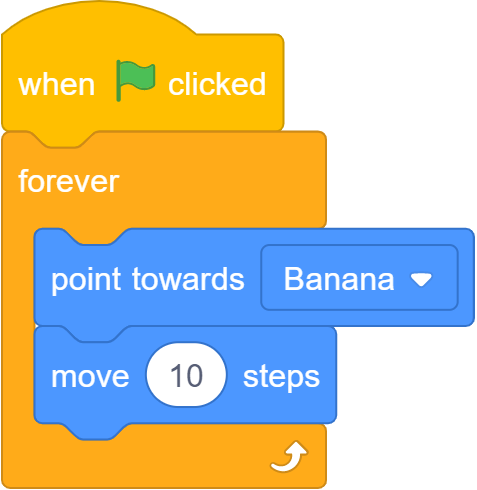
\includegraphics[width=5cm]{exampleTokens(1).png}\label{fig:exampleTokens(1)} }}%
    \qquad
    \subfloat[Second script of monkey sprite]{{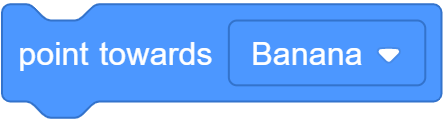
\includegraphics[width=5cm]{exampleTokens(2).png}\label{fig:exampleTokens(2)} }}%
    \caption[Example bug detection with \ngram{}]{\label{fig:exampleTokens}Example bug detection with \ngram{}}%
\end{figure}

In this bachelor's thesis a technique that uses \ngram{s} to automatically detect bugs in \scratch{} programs is proposed. For instance, Figure~\ref{fig:exampleTokens} shows \scratch\ scripts that were created as a solution for the \textit{Monkey} task and control the monkey sprite in the project. 

The block sequence [Never, GoToPos], shown in Subfigure~\ref{fig:exampleTokens(2)}, can basically never be executed because of a missing \textit{hat block}. Consequently, it is a rather unusual sequence and has only a probability of 0.12\%, whereas the sequence [GreenFlag, RepeatForeverStmt], which can be found as the first two blocks in Subfigure~\ref{fig:exampleTokens(1)}, is a common use case with an occurrence probability of 7.18\%. Therefore, the sequence [Never, GoToPos] is suspicious and indicates the existence of a code smell or bug. 

This is an example of how to use the \ngram\ to find low probability sequences and mark them as potential bugs that should be further analysed by the programmer. The accuracy of the probability calculation depends on many configuration parameters of the model and calculation methods like \hyperref[def:smoothing]{\textit{smoothing}} that will be explained further in this bachelor's thesis. 
